\chapter{Intégration temporelle}

\paragraph{}
Nous avons vu dans l'introduction que lorsqu'on résout un problème de simulation numérique de la dynamique des fluides, on se ramène à résoudre une équation différentielle ordinaire de la forme (\ref{eq:edo}).
Il existe différents algorithmes permettant de résoudre une telle équation, et la plupart de ces algorithmes se rangent dans deux catégories : les méthodes explicites, et les méthodes implicites.

\section{Analyse des méthodes}

  \paragraph{}
  Il est nécessaire de définir quelques notions pour pouvoir analyser les méthodes qui vont suivre.

  \section{Consistance et ordre}

    \paragraph{}
    Une méthode de résolution d'équations différentielles doit respecter certaines propriétés pour être "correcte".
    Notamment elle se doit d'être consistante.
    Pour définir cette notion, on se place dans le cadre de l'équation (\ref{eq:edo}).
    Après un pas, la méthode numérique donne une valeur $W_1$ que l'on souhaite proche de la valeur exacte $W\left(t_0 + \Delta\right)$.
    La méthode est dite consistante si :
    \[\lim_{\Delta t \rightarrow 0} \frac{W_1 - W\left(t_0 + \Delta t\right)}{\Delta t} = 0\]

    \paragraph{}
    De plus, on dira que la méthode est d'ordre $p$ si l'erreur locale est en $\Delta t^{p+1}$ :
    \[W_1 - W\left(t_0 + \Delta t\right) = O\left(\Delta t^{p+1}\right)\]


  \section{Stabilité}

    \paragraph{}
    Un critère important dans le choix d'une méthode d'intégration est la stabilité.
    En fonction de notre cas d'application, on exigera certains niveaux de stabilité pour éviter une divergence d'origine numérique du calcul.
    Nous cherchons dans cette section à analyser la stabilité d'une méthode d'intégration de l'équation (\ref{eq:edo}).
    Pour simplifier, on considère ici que le pas de temps $\Delta t = t_{n+1} - t_n$ ne dépend pas du numéro de l'itération $n$.
    La taille du problème est notée $N$.

    \paragraph{}
    Pour étudier la stabilité d'une méthode, on utilise en général l'équation différentielle ordinaire avec un second membre linéaire \cite{HairerWanner1996}.
    En effet, si on dispose d'une solution $\tilde{W}$ de (\ref{eq:edo}), on peut linéariser $F$ en $\tilde{W}$ :
    \[\frac{\mathrm{d}W}{\mathrm{d}t} = F\left(\tilde{W}\right) + \frac{\partial F}{\partial W}\left(\tilde{W}\right)\cdot\left(W - \tilde{W}\right)\]
    Si on note ensuite $y = W - \tilde{W}$ et $A = \frac{\partial F}{\partial W}\left(\tilde{W}\right)$, on obtient :
    \begin{equation}\label{eq:stab}
      \frac{\mathrm{d}y}{\mathrm{d}t} = Ay
    \end{equation}
    C'est donc avec cette équation, également appelée équation de Dahlquist, que l'on étudie la stabilité de la méthode.
    Nous l'étudions dans $\mathbb{C}$.

    \paragraph{}
    Pour une méthode d'intégration donnée, on note :
    \begin{equation}\label{eq:stab_req}
      y_{n+1} = G\left(\Delta tA\right)y_n
    \end{equation}
    la relation qui donne l'état suivant en fonction de l'état actuel.
    Pour la plupart des méthodes d'intégration temporelle, et en particulier pour les méthodes de Runge-Kutta présentées ici, on peut se ramener à cette écriture avec $G$ une fonction analytique.
    On peut choisir une base de vecteurs propres de $A$ $v_1, \dots, v_N$ associés aux valeurs propres $\alpha_1, \dots, \alpha_N$.
    Si on décompose l'itéré initial sur cette base, c'est à dire $y_0 = \sum_{i=1}^N\lambda_iv_i$, on voit que puisque $G$ est une fonction analytique :
    \[y_n = \sum_{i=1}^N\lambda_iG\left(\Delta t\alpha_i\right)^nv_i\]

    \paragraph{}
    Il découle de l'équation précédente que si $G\left(\Delta t\alpha_i\right)^n$, alors $y_n$ tend vers 0.
    C'est ainsi qu'on définit le domaine de stabilité d'une méthode d'intégration temporelle :
    \[\left\{\,z\in\mathbb{C}\;\mid\;\left|G\left(z\right)\right| < 1\,\right\}\]
    Si toutes les valeurs propres de $A$ sont à partie réelle négatives, alors la solution de l'équation (\ref{eq:stab}) converge vers 0.
    On comprend alors tout de suite que pour que l'algorithme soit stable, il faut que les valeurs propres de $A$ soient toutes dans le domaine de stabilité de la méthode.

    \paragraph{}
    On remarque que l'argument de $G$ n'est pas $A$ mais $\Delta tA$.
    Si une valeur propre $\Delta t\alpha_i$ de $\Delta tA$ n'est pas dans le domaine de stabilité de la méthode, la direction propre associée sera amplifiée et une instabilité d'origine numérique entraînera la divergence du calcul.
    On va donc jouer sur la valeur de $\Delta t$ : en la prenant assez faible, on arrivera à faire rentrer toutes les valeurs propres dans le domaine de stabilité, et donc à garantir la stabilité du calcul.
    Cependant, comme nous le verrons par la suite, cela impose l'utilisation de pas de temps relativement faible, ce qui s'avère contraignant pour nos application.

    \paragraph{}
    La propriété clef découlant de cette étude de stabilité est la "A-stabilité" \cite{Dahlquist1963}.
    Une méthode d'intégration temporelle est dite A-stable si son domaine de stabilité inclut le demi-plan des complexe à partie réelle négative.
    Autrement dit, une méthode est A-stable si elle converge bien vers 0 lorsqu'elle le devrait, et ne fait donc pas diverger l'erreur numérique.


\section{Méthodes explicites}

  \paragraph{}
  Les méthodes explicites cherchent l'état suivant $W_{n+1}$ en fonction des états précédents :
  \[W_{n+1} = F_e\left(W_n, W_{n-1}, \dots, W_0\right)\]
  Ces méthodes sont généralement utilisées dans les simulations numériques instationnaires de la dynamique des fluides.
  L'avantage de ces méthodes est d'une part leur facilité d'implémentation, et d'autre part leur faible coût numérique.
  En effet, puisque l'état recherché est accessible à partir des états précédents, la seule écriture d'une fonction est nécessaire au développement de la méthode, et le coût numérique à chaque itération se résume à l'évaluation de cette fonction.

  \subsection{Méthode d'Euler}

    \paragraph{}
    La méthode d'Euler, ou Euler explicite, est la méthode la plus simple qui soit.
    Elle consiste à intégrer (\ref{eq:edo}) entre $t_n$ et $t_{n+1} = t_n + \Delta t$ en supposant le second membre constant égal à $F\left(W_n\right)$, ou de manière équivalente à remplacer la dérivée dans (\ref{eq:edo}) par le taux d'accroissement : $\frac{\mathrm{d}W}{\mathrm{d}t}\approx\frac{W_{n+1}-W_n}{\Delta t}$.
    Ainsi, cette méthode donne la relation de récurrence explicite :
    \[W_{n+1} = W_n + \Delta t F\left(W_n\right)\]

    \paragraph{}
    Lorsqu'on réalise l'analyse de stabilité de cette méthode, on voit que la fonction $G$ de l'équation (\ref{eq:stab_req}) est $z\mapsto 1 + z$.
    Dans le plan complexe, son domaine de stabilité est donc le disque unité ouvert centré en -1.
    En pratique, ce domaine de stabilité s'avère insatisfaisant car il prohibe l'utilisation de grands pas de temps.


  \subsection{Méthodes de Runge-Kutta}

    \paragraph{}
    Les méthodes de Runge-Kutta forment une classe de méthodes qu'on appellera "multi-étapes", pour établir un contraste avec les méthodes "multi-pas" présentées plus bas.
    Plutôt que de faire un unique pas en avant comme le fait la méthode d'Euler explicite, on va réaliser un ensemble de pas intermédiaires, le pas final étant une combinaison de ces pas intermédiaires.

    \paragraph{}
    Le principe général est le suivant.
    En supposant qu'en $t_n$ on dispose d'une valeur de la solution $W_n$, on introduit les étapes intermédiaires $t_{n,i} = t_n + c_i\Delta t$ pour $1\leq i\leq k$, avec $k$ fixé.
    On peut intégrer entre $t_n$ et $t_{n,i}$ l'équation (\ref{eq:edo}) de manière exacte :
    \[W\left(t_{n,i}\right) = W\left(t_n\right) + \Delta t \int_0^{c_i}F\left(W\left(t_n + s\Delta t\right)\right)\mathrm{d}s\]
    L'intégrale est ensuite approchée par une quadrature sur les points $j<i$ :
    \[\int_0^{c_i}F\left(W\left(t_n + s\Delta t\right)\right)\mathrm{d}s \approx \sum_{j = 1}^{i-1}a_{ij}F\left(W\left(t_{n,j}\right)\right)\]
    Les étapes déjà calculées permettent donc de calculer la quadrature afin d'obtenir l'étape suivante.
    Une fois qu'on a obtenu toutes les étapes intermédiaires, on intègre (\ref{eq:edo}) entre $t_n$ et $t_{n+1}$ :
    \[W_{n+1} = W_n + \Delta t \int_0^1F\left(W\left(t_n + s\Delta t\right)\right)\mathrm{d}s\]
    que l'on approche de nouveau par la quadrature :
    \[\int_0^1F\left(W\left(t_n + s\Delta t\right)\right)\mathrm{d}s \approx \sum_{i = 1}^kb_iF\left(W\left(t_{n,i}\right)\right)\]

    \paragraph{}
    Une méthode de Runge-Kutta est donc caractérisée par sa taille $k$ et par les valeurs $a_{ij, 1\leq j<i\leq k}$, $b_{i, 1\leq i\leq k}$ et $c_{i, 1\leq i\leq k}$.
    Ces valeurs de quadrature sont souvent représentées dans le tableau de Butcher :
    \[\begin{array}{c|ccccc}
      0\\
      c_2    & a_{21} \\
      c_3    & a_{31} & a_{32} \\
      \vdots & \vdots &        & \ddots\\
      c_k    & a_{k1} & a_{k2} & \hdots & a_{k,k-1}\\
      \hline & b_1    & b_2    & \hdots & b_{k-1} & b_k
    \end{array}\]

    On rappelle ici les tableau de Butcher des méthodes les plus connues :
    \begin{table*}[h]\begin{tabular}{P{.15\textwidth}P{.3\textwidth}P{.4\textwidth}}
      \begin{tabular}{c|c}
        0 \\ \hline & 1
      \end{tabular} &
      \begin{tabular}{c|cc}
        0 \\ 1/2 & 1/2 \\ \hline & 0 & 1
      \end{tabular} &
      \begin{tabular}{c|cccc}
        0 \\ 1/2 & 1/2 \\ 1/2 & 0 & 1/2 \\ 1 & 0 & 0 & 1 \\ \hline & 1/6 & 1/3 & 1/3 & 1/6
      \end{tabular} \\
      RK1 & RK2 & RK4 \\
    \end{tabular}\end{table*}

    \paragraph{}
    La méthode RK1 est équivalente à la méthode Euler explicite présentée précédemment.
    Cette méthode RK2 est également appelée méthode du point milieu.
    Cette méthode RK4 est d'ordre 4, et est l'une des plus utilisées pour l'intégration explicite des équations différentielles.

    \paragraph{}
    On peut montrer que l'ordre de la méthode $p$ est tel que $p \leq k$.
    Jusqu'à $k = 4$ on a $k = p$.
    Pour les ordres supérieurs, obtenir une borne entre l'ordre et la taille de la méthode est encore un problème ouvert.
    Pour une méthode de Runge-Kutta d'ordre $p$, la fonction $G$ de l'équation (\ref{eq:stab_req}) est telle que \cite{HairerWanner1996}:
    $$G\left(z\right) = 1 + z + \frac{z^2}{2} + \dots + \frac{z^p}{p!} + O\left(z^{p+1}\right)$$
    Lorsque la méthode est telle que l'ordre $p$ est égal à la taille $k$, le terme en $O\left(z^{p+1}\right)$ est nul.
    On peut donc tracer sur la figure \ref{fig:rk_stab} les domaines de stabilité des méthodes de Runge-Kutta.

    \begin{figure}
      \centering
      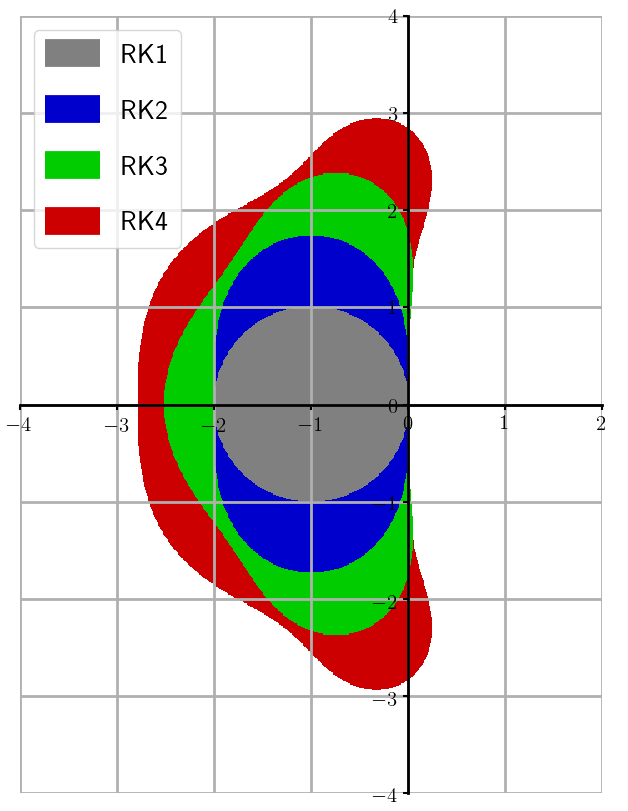
\includegraphics[width=.5\textwidth]{images/rk_stab.png}
      \caption{Domaines de stabilité (en couleur) des méthodes de Runge-Kutta pour les quatre premiers ordres.}
      \label{fig:rk_stab}
    \end{figure}

    \paragraph{}
    On constate alors que les méthodes de Runge-Kutta ne sont pas A-stables, et en particulier n'ont pas un large domaine de stabilité.
    En pratique, cela imposera l'utilisation de faibles pas de temps, chose acceptable pour des calculs instationnaires mais insatisfaisante pour nos calculs stationnaires.
    Si le coût de la méthode est moindre, le nombre d'itérations nécessaires pour converger vers un état stationnaire va rendre le coût de calcul global trop important.


  \subsection{Méthodes d'Adams-Bashforth}

    \paragraph{}
    Les méthodes d'Adams-Bashforth sont des méthodes de type "multi-pas" (multi-step), c'est à dire qu'elles utilisent plusieurs états précédents pour déterminer l'état suivant.
    A la différence des méthodes de Runge-Kutta qui utilisent des pas intermédiaires entre $t_n$ et $t_{n+1}$, ces méthodes utilisent les $t_{i\leq n}$ précédents.
    Pour une méthode d'ordre $k$, on utilise donc les états $W_n, \dots, W_{n-k+1}$ pour déterminer $W_{n+1}$.
    On peut en effet vérifier que pour ces méthodes, l'indice $k$ désignant la méthode est égal à l'ordre de la méthode \PS{Apparemment dans "Solving ordinary differential equations I: Nonstiff problems", à citer si j'arrive à le trouver}.

    \paragraph{}
    L'idée est d'interpoler le second membre de (\ref{eq:edo}) en ces $k$ points calculés précédemment.
    Il existe en effet un unique polynôme $F_k$ tel que pour $0 \leq i < k$ on ait $F_k\left(t_{n-i}\right) = F\left(W_{n-i}\right)$.
    On fait ensuite l'hypothèse $F_k\left(t\right) \approx F\left(W\left(t\right)\right)$.
    On peut intégrer l'équation (\ref{eq:edo}) :
    \[W_{n+1} = W_n + \int_{t_n}^{t_{n+1}}F_k\left(t\right)\mathrm{d}t\]

    \paragraph{}
    Contrairement aux méthodes de Runge-Kutta, puisqu'on réutilise les pas précédents, une unique évaluation du second membre de (\ref{eq:edo}) est nécessaire à chaque itération.
    Le coût de calcul est donc très faible pour de telles méthodes.
    Cependant, les propriétés de stabilité de ces méthodes sont moindres, ce qui explique le fait qu'elles ne sont pas souvent utilisées en pratique dans des codes de calcul pour la dynamique des fluides.

    \paragraph{}
    Les méthodes d'Adams-Bashforth, et plus généralement les méthodes multi-pas, ne rentrent pas dans le cadre d'étude de la stabilité présenté précédemment.
    L'analyse de leur stabilité est plus complexe, \cite{HairerWanner1996} \PS{cter également "Solving ordinary differential equations I: Nonstiff problems"} et ne sera donc pas détaillé ici.
    Cependant, on constate que la stabilité de ces méthode est en général de l'ordre des méthodes de Runge-Kutta.
    De manière générale, il n'existe pas de méthodes multi-pas explicites qui sont A-stables.


\section{Méthodes implicites}
